In this appendix, we provide \edit{an example datasheet for}
Pang and Lee's
polarity dataset~\cite{polarity} (figure~\ref{fig:polarity1} to
figure~\ref{fig:polarity4}).

\begin{figure*}[p]
  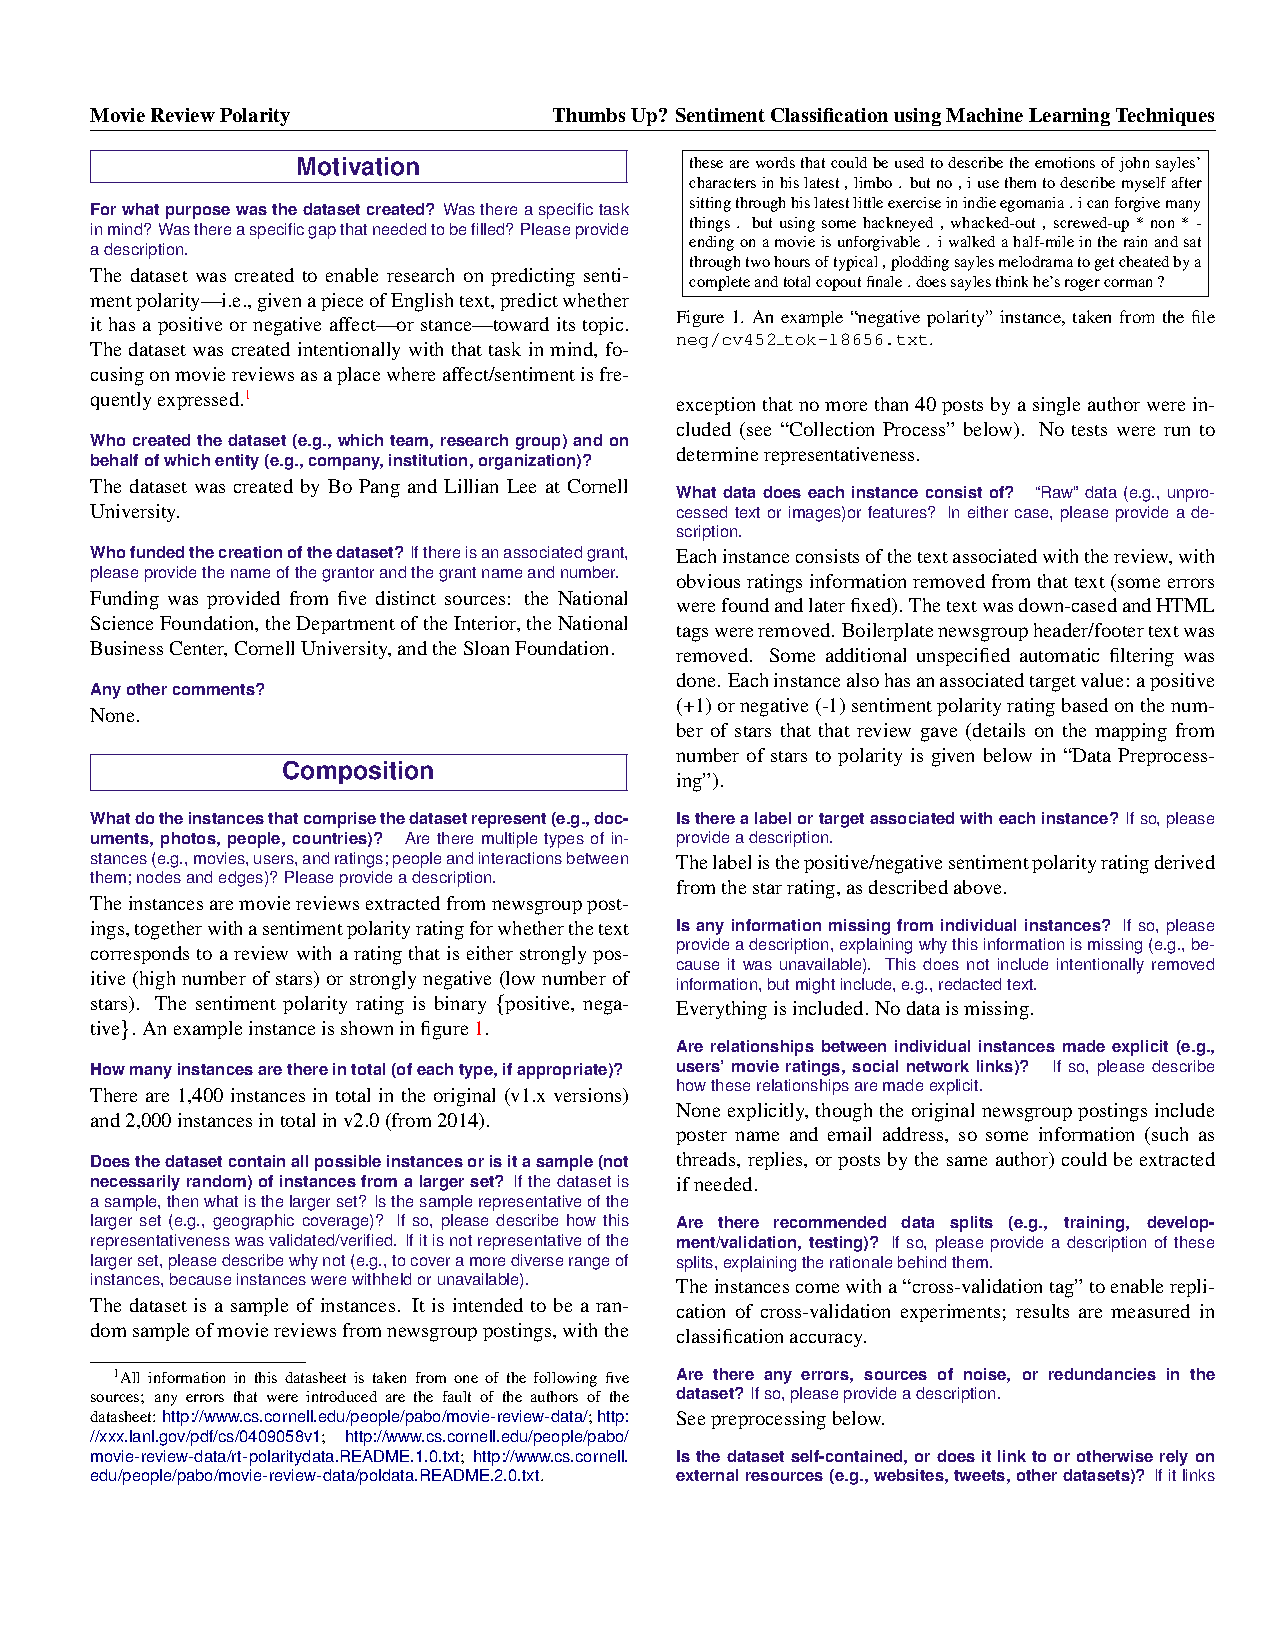
\includegraphics[page=1,width=1.0\textwidth]{datasheet_sentiment.pdf}
  \caption{\label{fig:polarity1}Example datasheet for Pang and Lee's
    polarity dataset~\cite{polarity}, page 1.}
  \vspace{-1cm}
\end{figure*}

\begin{figure*}[p]
  \includegraphics[page=2,width=1.0\textwidth]{datasheet_sentiment.pdf}
  \caption{\label{fig:polarity2}Example datasheet for Pang and Lee's
    polarity dataset~\cite{polarity}, page 2.}
  \vspace{-1cm}
\end{figure*}

\begin{figure*}[p]
  \includegraphics[page=3,width=1.0\textwidth]{datasheet_sentiment.pdf}
  \vspace{-1cm}
  \caption{\label{fig:polarity3}Example datasheet for Pang and Lee's
  polarity dataset~\cite{polarity}, page 3.}
\end{figure*}

\begin{figure*}[p]
  \includegraphics[page=4,width=1.0\textwidth]{datasheet_sentiment.pdf}
  \vspace{-1cm}
  \caption{\label{fig:polarity4}Example datasheet for Pang and Lee's
  polarity dataset~\cite{polarity}, page 4.}
\end{figure*}
